\chapter{Evaluation} \label{chapter:EVALUATION}

We evaluated our implementation of version-aware references in terms of functionality and practicability, as presented and discussed in this Chapter.
Regarding functionality, we evaluated whether our proxy-based version-aware references behave correctly like particular versions and whether they allow to preserve and re-establish versions of the development state in the Lively Kernel.
Regarding practicability, we evaluated the impact of proxy-based version-aware references on both memory consumption and execution speed.
For this evaluation, we used a standard benchmark suite and the Lively Kernel.


\section{Test Setup}

We tested the implementation of version-aware references with a standard JavaScript benchmark suite and with the target programming system, the Lively Kernel.
For all tests, we used the test machine described in this section.


\subsection{The Octane JavaScript Benchmark Suite}

% what?
We used the \emph{Octance} benchmark suite\footnote{\url{http://code.google.com/p/octane-benchmark/}, accessed February 3, 2014, at version 26} to test both the behavior and performance overhead of our alternative references.
Octane is a general JavaScript benchmark suite that consists of eight benchmarks.
It does not test JavaScript's language features systematically, but instead is a benchmark suite of programs such as the \emph{DeltaBlue}\cite{FreemanBenson1990ICS} constraint solver.
These selection of JavaScript programs do, however, make use of many important language features, including primitive data types, operators, built-in functions, custom functions, objects, and prototypical inheritance.
Octane advertises itself as providing tests that are representative of modern Web applications.
It is also used in measuring the performance of \emph{v8}, the engine incorporated by both the Chrome browser and Node.js, and even part of its official source code repository\footnote{\url{http://v8.googlecode.com/svn/}, accessed April 23, 2014, at revision 20901}.

% why?
We decided to use the Octane suite for two reasons.
First, it covers many JavaScript language features and seems to be a benchmark suite that is widely in use.
Second, it is the JavaScript benchmark suite used by the Chrome browser, which is also the browser we used in both developing and testing our implementation.


\subsection{The Lively Kernel System}

% what?
We also used Lively Kernel itself to test the implementation of our approach in it.
We integrated our approach with the version 2.1.3 of the Lively Kernel and, in particular, used the commit ba726ddca08df66b775e904366cdcbd76c4920f6\footnote{\url{http://github.com/LivelyKernel/LivelyKernel/commits/ba726ddca08df66b775e904366cdcbd76c4920f6}, accessed February 17, 2014} as starting point for our changes.
The version we used for the tests described in this section is fc6f3b7e7e75cf3f866a8e5eb5899d65a5530654\footnote{\url{http://github.com/LivelyKernel/LivelyKernel/commits/fc6f3b7e7e75cf3f866a8e5eb5899d65a5530654}, accessed February 17, 2014}.
This version transforms most of the Lively Kernel's code to insert proxies for all references to mutable objects.
In particular, the versioning system is loaded and enabled right after loading Lively Kernel's module system, which excludes the extensions to the built-in JavaScript types, the bootstrap logic, and the module system itself, but includes everything loaded thereafter, including all actual modules of the Lively Kernel and, with that, also all classes.

% why?
We tested the Lively Kernel itself with our implementation for multiple reasons.
First, the Lively Kernel is a large JavaScript application that makes use of many features of both the JavaScript language but also the browser as particular host environment.
That is, it makes use of not only most of the features described in the language specification, including the language's standard library, but also much of the additional built-in functionality of the browser, which, for example, includes the built-in functions to manipulate the HTML document.
Second, the main goal of the presented work is to provide object versioning for the Lively Kernel, which just happens to be implemented in JavaScript.
Thus, we are particularly interested in evaluating our implementation with the JavaScript parts used by the Lively Kernel.


\subsection{Test Machine Configuration}

% what?
All tests and measurements were done on a Macbook Air with an 2 GHz Intel Core i7 and 8 GB main memory, using Mac OS X 10.9.1.
We further used the most recent stable release of the Chrome browser on February 18, 2014, which was version 32.0.1700.107.

The presented measurement results were averaged over five runs.

% why?
We used Chrome for all experiments as the Lively Kernel currently works best in Chrome.







\section{Functionality: Versions of the Lively Kernel Runtime} \label{sec:DISCUSSION:1}

We tested whether the version-aware references forward to particular versions correctly both with benchmarks and with the Lively Kernel, as described in this section, and did this continuously during the implementation of our approach.

\subsection{Testing with Benchmarks}

\paragraph{Method}
% what was done?
We ran the Octane benchmark suite to test the functionality of our implementation.
For this, we transformed the Octane benchmarks with our source transformations, executed the resulting code, and then checked for JavaScript errors as well as compared the results of the transformed benchmarks to their usual results.\\
% why / to test what?
We did this for to test two aspects.
First, to test whether our source transformations yield syntactically correct JavaScript code for the benchmarks.
Second, to test whether the proxy-based implementation of version-aware references, inserted by the source transformations, allows to run the benchmarks without errors and with the same results as when running the benchmarks without our implementation.


\paragraph{Results}
All benchmarks in this suite run without errors and return the same results as when executed without any source transformations.
That is, at least for these tests, our source transformations produce working source code and our proxy-based version-aware references behave as the object versions they refer to.
The benchmarks and, in particular, the \emph{DeltaBlue} benchmark revealed a problem with using proxies as prototypes of objects, which we reported to the \emph{harmony-reflect} repository\footnote{\url{http://github.com/tvcutsem/harmony-reflect/issues/18}, accessed April 23, 2014} and which turned out to be an issue with the \emph{v8} JavaScript engine itself\footnote{\url{http://code.google.com/p/v8/issues/detail?id=2804}, accessed April 23, 2014}.
We virtualized the prototype relation among proxies as workaround for this problem in our implementation, while the issue was subsequentely fixed, making the implemented workaround redundant.

\paragraph{Discussion}
The proxies, which implement version-aware references, behave like the respective versions of objects in the situations exhibited in the benchmarks.
While these benchmarks do not test JavaScript's features systematically, they cover a range of language features.


\subsection{Testing with the Lively Kernel}

\paragraph{Method}
% what was done?
We tested whether, when the Lively Kernel sources are transformed to use version-aware references, the Lively Kernel loads and works as expected.
We further tested whether the version-aware references and the linear global undo/redo that we built as explained in \todo{reference..} allow to preserve and re-establish versions of the Lively Kernel's JavaScript runtime in practice.
Here, we tried multiple example scenarios, including to undo changes to the state of simple morphs, morph compositions, and more complicated graphical applications as, for example, text editors and developer tools.\\
% why / to test what?
With this, we tested that the source transformations yield valid JavaScript code for the modules of the Lively Kernel, that the version-aware references delegate correctly to the versions of objects they stand-in for in Lively, and that the version-aware references are used consistently for all mutable objects.


\paragraph{Results}
The Lively Kernel does load when all of its modules are transformed to use version-aware references.
Further, most of its basic functionality works as expected and we were able to preserve and re-establish the particular runtime state of multiple example scenarios, as described above.
However, not all functionality works as expected and we were, thus, also not able to re-establish all preserved states. 
In particular, we did learn about the issues of the current implementation of the ECMAScript 6 through these experiments and implemented the workarounds described in Section~\ref{sec:IMPLEMENTATION:4}.

\paragraph{Discussion}
While most of the tested functionality of the the Lively Kernel---including the entire bootstrap process, rendering graphical objects, loading parts from the Lively Kernel's Parts Bin, and using the Lively Kernel's halo controls---work as expected with version-aware references, certain functionality of the Lively Kernel is not yet working correctly or even yield errors.
The remaining issues here are expected to be problems related to built-in JavaScript functions that do not handle proxies correctly.
Our implementation already unwraps proxies for many built-in functions, as explained in \ref{sec:IMPLEMENTATION:4}, but the configuration appears to not cover all problematic built-in functions, yet.
However, the used proxies are currently an experimental JavaScript feature in Chrome, not yet fully supported, and we expect these issues not to be problems once the proxies get fully supported by JavaScript engines.
Further, the current implementation already allows to re-establish many preserved development states of the Lively Kernel.




\section{Practicability: Effect on Memory Consumption} \label{sec:DISCUSSION:2}

% TODO: one-sentence section intro

\subsection{Memory Overhead for Version-aware References}

The version-aware references have an impact on memory consumption
focus on performance overhead of version-aware references, not of having multiple versions.. + why this? constant overhead for references, overhead for multiple versions dependent on the different versions.. but version-aware ref overhead a prerequisite for versions.. overhead of versions is also out of the scope of this thesis

% overhead ist erwartbar, aber die Frage, die sich stellt: ist der overhead vertretbar / das System mit version-aware references noch nutzbar / responsive?

% memory overhead for the version-aware references, not for preserving multiple versions

\paragraph{Method}
memory overhead for the version-aware references, not for preserving multiple versions
loading an empty the Lively Kernel world


\paragraph{Results}
As shown in Figure~\ref{fig:MemoryOverhead}, loading an empty the Lively Kernel world requires three times more space with proxies than without proxies.

\begin{figure}[h]
    \centering
    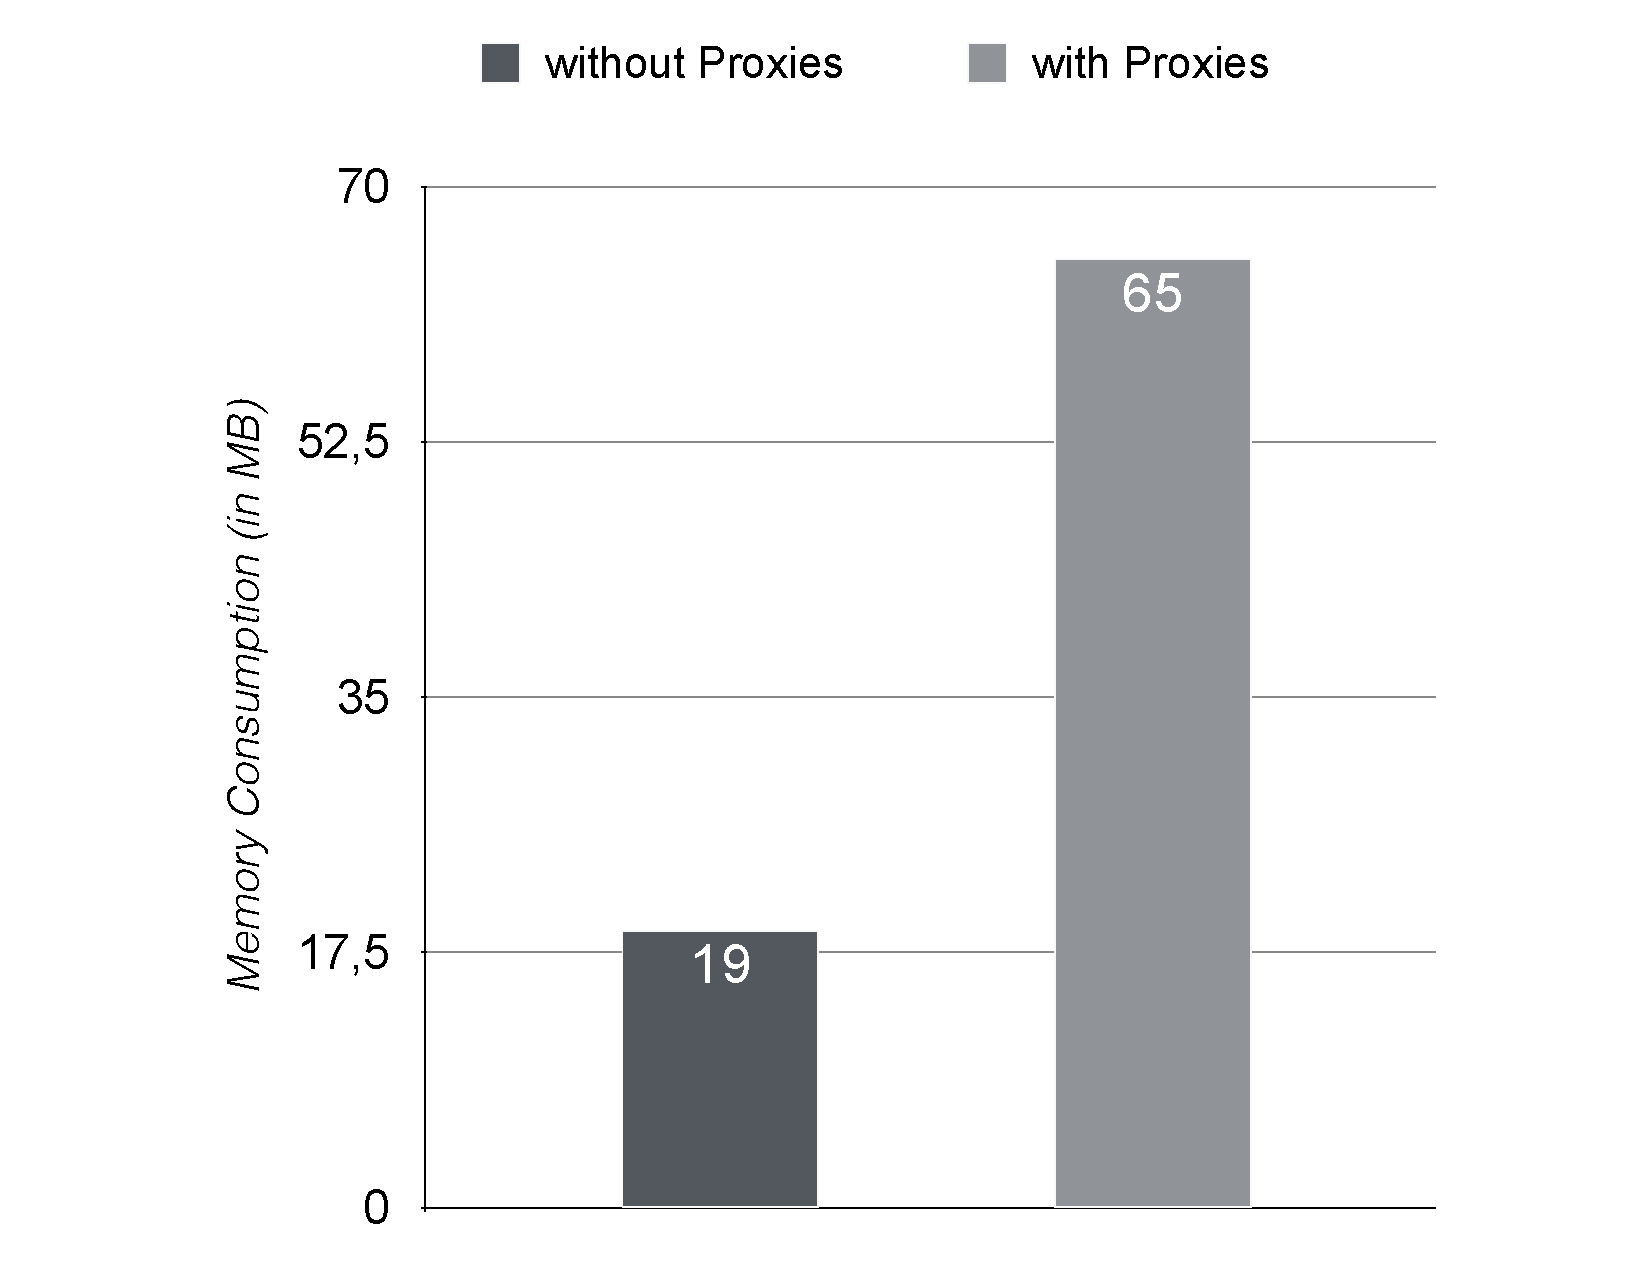
\includegraphics[width=\textwidth]{figures/6_evaluation/1_memoryOverhead.pdf}
    \caption{Memory consumption when starting an empty the Lively Kernel Kernel world in megabyte.}
    \label{fig:MemoryOverhead}
\end{figure}

\paragraph{Discussion}
The memory overhead of our implementation appears to be practical.

In our proxy-based implementation, the system uses a proxy for each reachable mutable object and all references that would usually refer directly to the object refer to the proxy instead.
These proxies require additional space.
That is, even without preserving multiple versions for any object, the system requires more space when all mutable state is referred to only through proxies.
For each proxied object the system now also has a proxy, which comprises of an internal proxy object, a proxy handler object that implements the proxy's behavior, an ordinary JavaScript object as dictionary for all available versions of the object the proxy stands-in for, and boolean flags to, for example, indicate whether a proxy should preserve versions at all or not.
While the system creates proxies for most objects, it does not use proxies for, for example, all objects created before our language-level implementation of object versioning is loaded and all objects used for implementing the versioning itself.




\subsection{Memory Usage for Preserving Versions}

\paragraph{Method}

\paragraph{Results}

\todo{present a heap measurement for a particular scenario, where multiple commits can be marked in the graph to show that for the versions only relatively little memory needs to be reserved / maybe also compared to the memory needed for opening a system code browser (or similar) in the same graph..}

\paragraph{Discussion}
In contrast to the memory overhead for the version-aware references, the memory consumption for preserving different versions of the runtime does not increase linearly with the number of proxied objects or even with the number of versions.
Our implementation does not copy all objects for each version, but only creates copies when objects change between versions, effectively storing only diffs on the granularity of objects.
Therefore, the memory required for new versions of the runtime depends on how many objects change and how big those objects are.
Thus, the memory overhead for preserving multiple versions of the the Lively Kernel runtime depends highly on concrete usage scenarios.





\section{Practicability: Impact on Execution Speed} \label{sec:DISCUSSION:3}

% TODO: one-sentence subsection intro

% TODO: 

In general, the experienced slow down does not depend as much on the number of preserved versions as it is dependent on how many version-aware references have to be resolved during the execution of particular code.
As versions of objects are created only when objects change between versions, preserving a version of the runtime happens incrementally and not at a single moment in time.
Additionally, changing a version also does not take significant time as the version-aware references are not updated but dynamically delegate differently the next time they are resolved.
To give an impression on how the version-aware references, however, impact the execution speed in general, we compared using the proxies to not using the proxies for both the Octane benchmark suite and a few particular typical user interactions in the Lively Kernel.
Additionally, a microbenchmark shows how much more time is necessary to resolve a single proxy-based version-aware reference.


\subsection{Measuring Benchmarks}

\paragraph{Method}
Octane benchmarks\footnote{Note: We reduced the input size to the Splay benchmark by an order of magnitude to prevent the browser from prompting for user input during the benchmarks execution. This prompt is a reaction to the long time required to run the benchmark, cannot be disabled, and would influence the benchmark result.}

\paragraph{Results}
Figure~\ref{fig:ExecutionOverhead} shows how much more time the benchmarks take when their source is transformed before execution and references are, therefore, version-aware.
Executing the benchmarks takes between 90 and 405 times longer with version-aware references than without.
On average the slowdown of a single benchmark is, thus, a 187.5 times.

\begin{figure}[h]
    \centering
    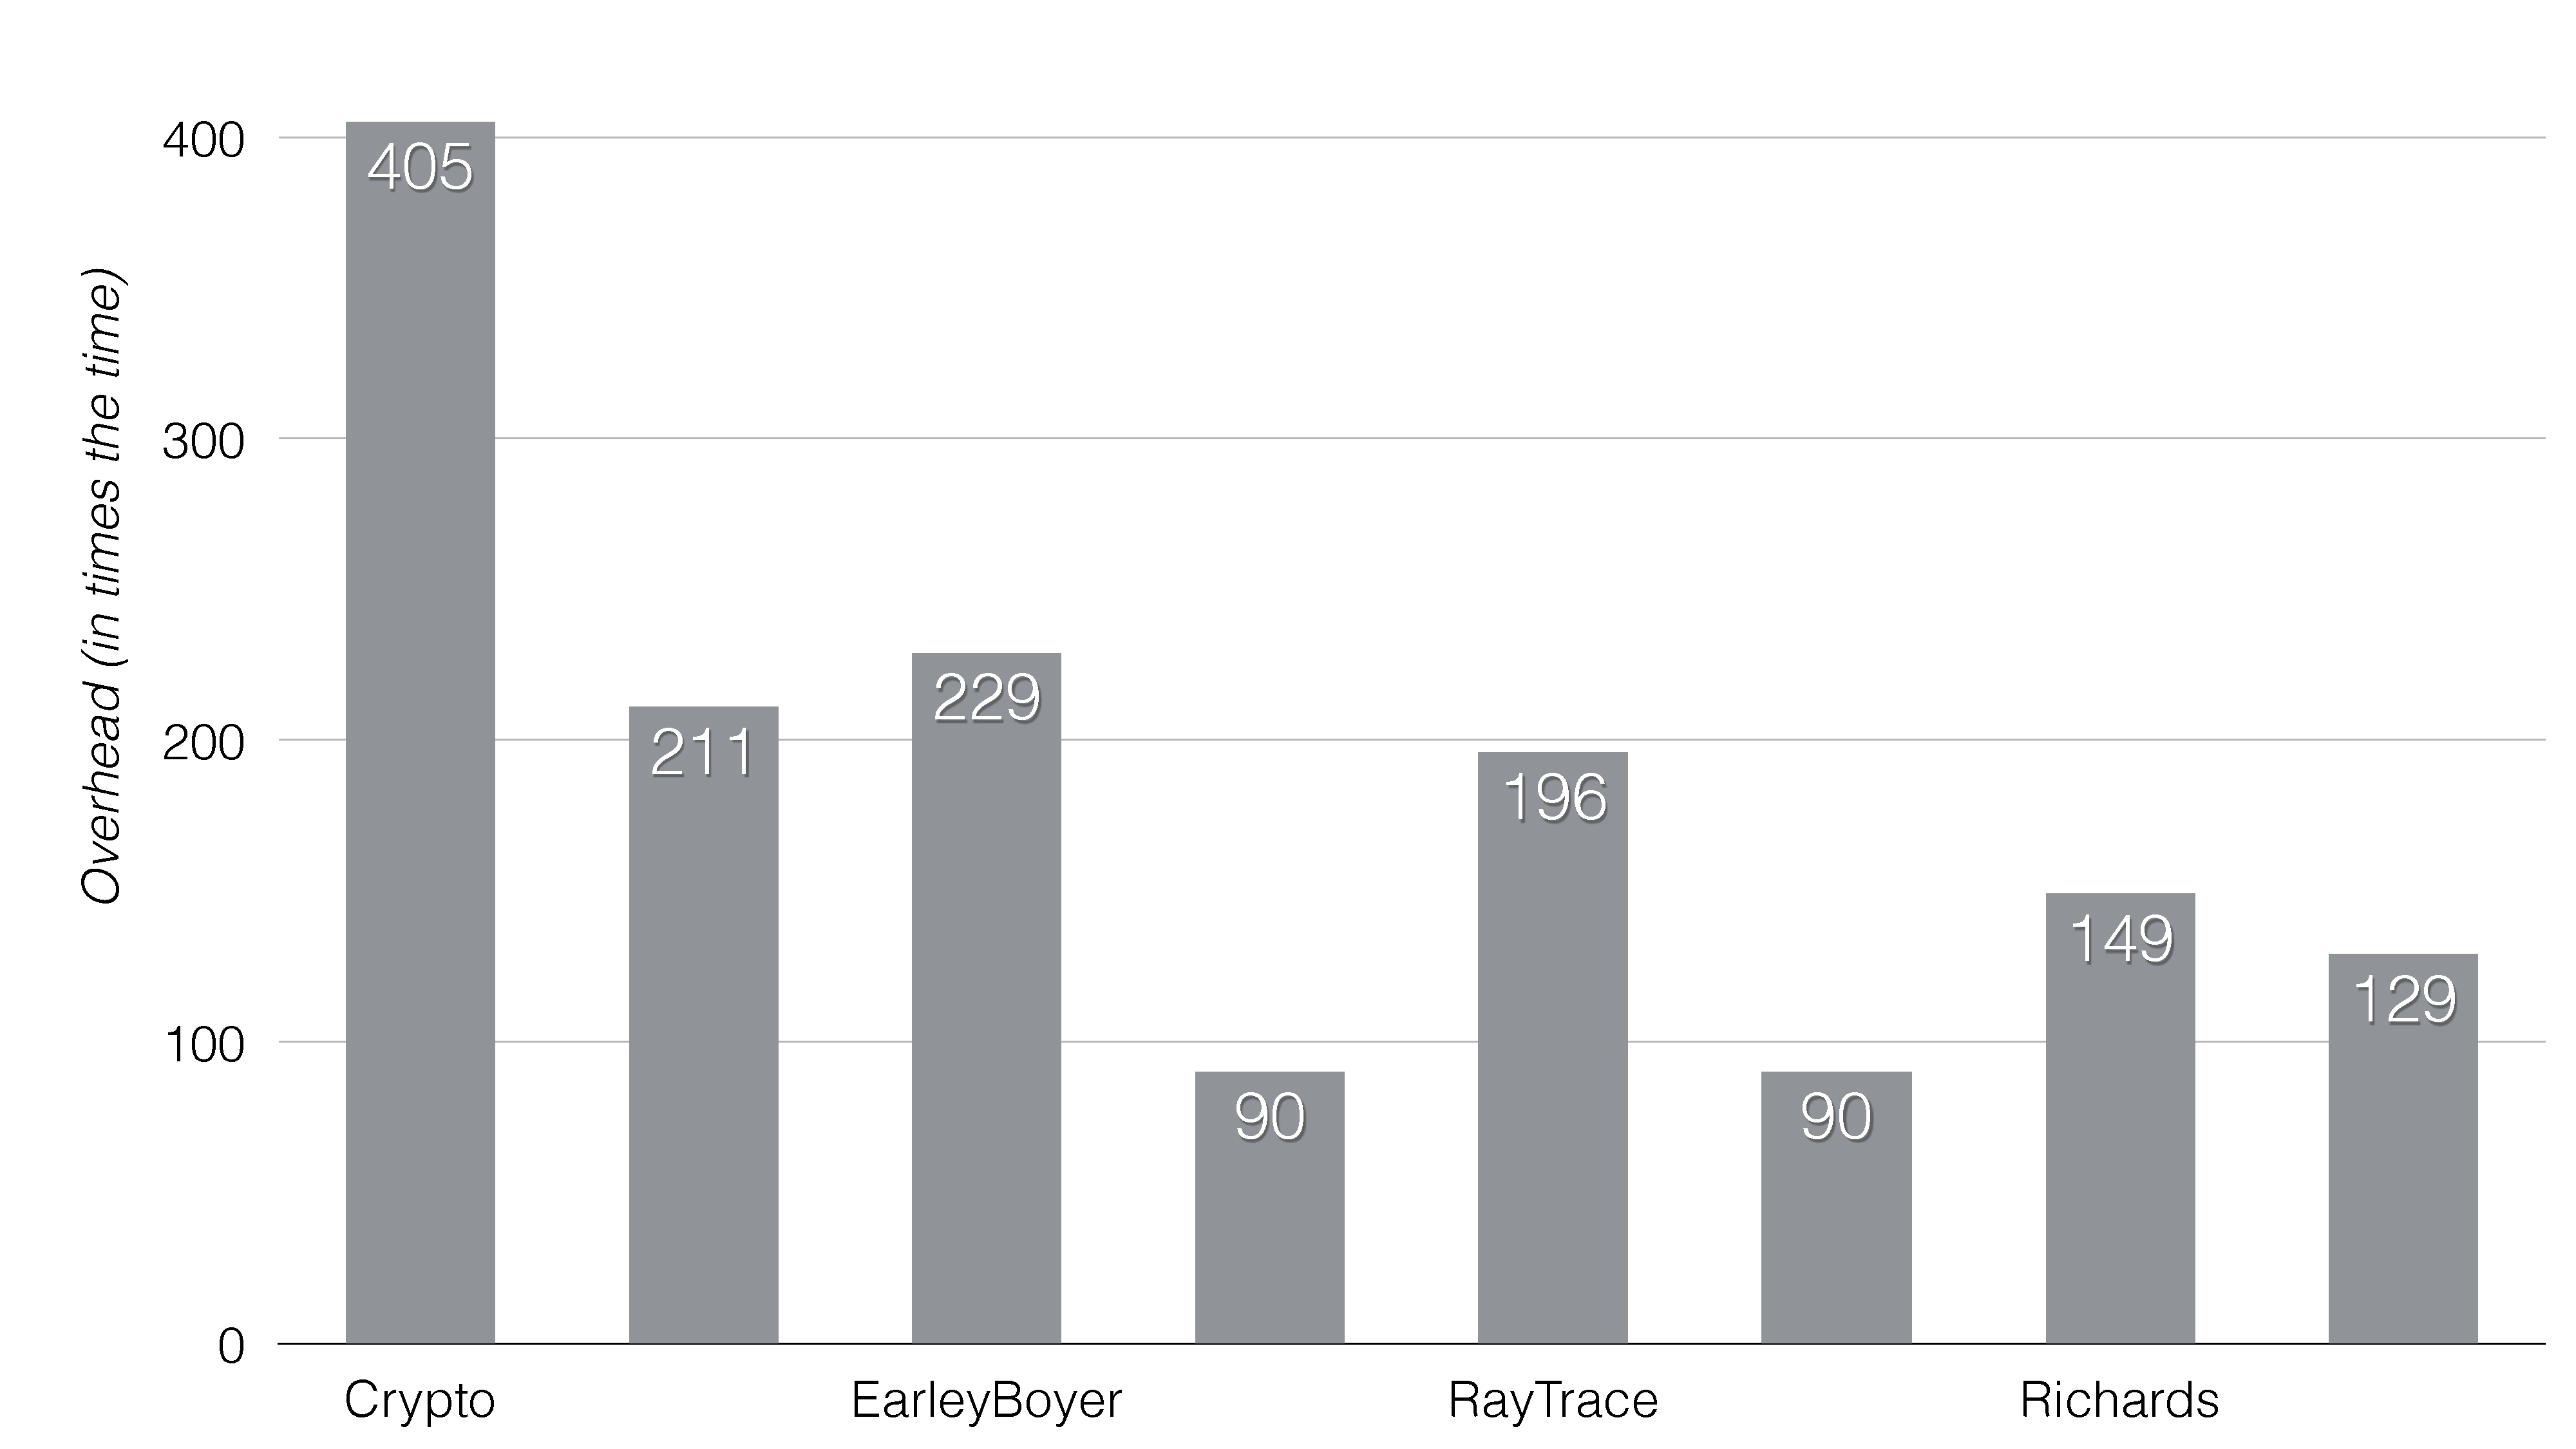
\includegraphics[width=\textwidth]{figures/6_evaluation/2_executionOverhead.pdf}
    \caption{Execution overhead for proxy-based version-aware references in 100\% overhead compared to ordinary JavaScript references.}
    \label{fig:ExecutionOverhead}
\end{figure}

\paragraph{Discussion}
% TODO: distinct paragraphs for approach / method (what was done? why / to test what?), results, discussion



\subsection{Measuring the Lively Kernel}

\subsubsection{the Lively Kernel interactions..}

While object versioning could be used for undo and redo in a specific application, it is primalary itented to support development and similar explorative tasks.
That could, conceivably, be an argument for providing object versioning only during development and not when programs should run at full speed.
However, besides having the disadvantage of introducing distinct usage modes, this still requires the version-aware references to resolve fast enough to not impede development significantly.

\paragraph{Method}
Therefore, in addition to measuring the execution of general JavaScript programs, we also measured the overhead for typical user interactions in the Lively Kernel.
...a direct comparison between using proxies and not using proxies for three selected user interactions: bringing up the halo buttons on a particular morph, opening the world's menu, and opening the Lively Kernel's System Code Browser.


\paragraph{Results}
Figure \ref{fig:LivelyInteractionsOverhead} shows ...
The three presented interactions are among the more impacted interactions compared to, for example, interactions are more browser-supported such as dragging a morph around.
All three interaction trigger code from multiple different modules, including event handling code, rendering code, and tool-specific code.

\begin{figure}[h]
    \centering
    \includegraphics[width=\textwidth]{figures/6_evaluation/3_LivelyInteractionsOverhead.pdf}
    \caption{Execution overhead for selected user interactions in the Lively Kernel in 100\% overhead.}
    \label{fig:LivelyInteractionsOverhead}
\end{figure}


\subsubsection{Loading a World in the Lively Kernel}

\paragraph{Method}
Another performance related question specific to the Lively Kernel is how long it takes to load a world.
This includes requesting the required modules from the Lively Kernel's server, but also client-side code to resolve dependencies among modules, evaluating all loaded modules, and deserializing a the Lively Kernel world.
In addition, in the case that version-aware references should be used, all required modules also need to be transformed.

\paragraph{Results}
The difference between providing object versioning and not is here a factor of around eight for loading a world: instead of around 4 seconds, the user would have to wait around 32 seconds until the requested the Lively Kernel world reacts on user interactions.



\subsection{Discussion of the Execution Overhead}


The execution overhead of the current implementation of version-aware referecens does not appear practical.

the current implementation slows down the JavaScript execution considerably: the benchmark programs need two to three orders of magnitude more time to finish, while particular typical user interactions in the Lively Kernel also take two orders of magnitude more time.

% The measured execution overhead is in the range of three orders of magnitude for popular JavaScript benchmarks and typical user interactions in the Lively Kernel.
% Direct comparisons of just the version-aware references and direct references in a microbenchmark even show slow downs of four orders of magnitude.

As this slowdown is due to the proxy-based version-aware references,

As explained in Section~\ref{sec:IMPLEMENTATION:1}, the proxies are currently implemented using a library that relies on an experimental implementation of a previous, deprecated draft of the proxy specification.
The proxies are also part of a ECMAScript specification that has not yet been finalized and completely implemented.


 we also implemented microbenchmarks to analyze exactly how long it takes to resolve such a reference.
When two objects are either connected by a proxy-based version-aware or a direct reference and this connection is resolved a million times to call a simple function, the microbenchmark takes three orders of magnitude more time when using the version-aware references: instead of on average ten milliseconds the test requires on average about 11000 milliseconds.
When we exchange the proxy-based version-aware reference for this benchmark with just a proxy, which then falls back on the default proxy behavior and not our specific versioning behavior, the difference is an order of magnitude less: using a direct reference still requires around 10 milliseconds, while placing a proxy in-between both objects requires close to 2000 milliseconds.
That is, even without our specific proxy behavior, the proxies slow down the microbenchmark close to 200 times.


% In analyzing these results, we gained the impression that only one order of magnitude is due to the specific proxy behavior, while most of the overhead can be ascribed to the Direct Proxies as currently available in the Chrome browser.



% In fact, a comparable indirection can be implemented considerably faster with ordinary JavaScript.

Further, similar indirections of object access as the default proxy handler provide could be implemented in JavaScript.
Instead of using a proxy for an object, we could still refer only to a stand-in, but implement the proxy behavior in an ordinary JavaScript function to which we would transform the source code: instead of \lstinline{obj.prop} we could execute something similar to \lstinline{get(obj, \"name\")}, where \lstinline{get} could implement the behavior previously implemented by respective the proxy trap.
Measuring the performance of such a manually provided indirection results in a much lower performance decrease for the previously described microbenchmark setup.
In fact, such an indirection would only take twice the time to read a property from a specific target using such a \lstinline{get}-function as it takes when reading a property directly. 
% Using such a custom JavaScript indirection and further source transformations, thus, promises a practical implementation.


All this suggests that the performance of the ECMAScript 6 Direct Proxies in Chrome might improve in the future.
At the same time, as suggested in Section~\ref{sec:FUTURE_WORK:1}, we might also decide to base our version-aware references on source transformations and custom indirections instead of proxies in the future.
